
%# -*- coding:utf-8 -*-
\documentclass[UTF8]{ctexart}
\usepackage{amsmath}
\usepackage{graphicx}
\setlength{\parindent}{0em}
\begin{document}

\section{解析几何}
曲线$\Gamma $ 在点P处的切向量为
$ \tau =
\begin{Bmatrix}

\begin{vmatrix}
F'_y & F'_z \\
G'_y & G'_z
\end{vmatrix}
,
\begin{vmatrix}
F'_z & F'_x \\
G'_z & G'_x
\end{vmatrix}
,
\begin{vmatrix}
F'_x & F'_y \\
G'_x & G'_y
\end{vmatrix}
\end{Bmatrix}
$

\section{两异面直线的距离}
$ d= \frac{ (\tau_1 \times \tau_2)\cdot \overrightarrow{P_1 P_2}}{\tau_1 \times \tau_2} = \frac{\begin{Vmatrix}
x_2-x_1 & y_2-y_1 & z_2-z_1 \\
l_1 & m_1 & n_1 \\
l_2 & m_2 & n_2
\end{Vmatrix}}{\begin{Vmatrix}
  i & j & k \\
  l_1 & m_1 & n_1 \\
  l_2 & m_2 & n_2
\end{Vmatrix}}
$

\section{解题技巧}
$\int_0^\pi xf(\sin x ) dx = \frac{\pi}{2} \int_0^\pi f(\sin x) dx$ \\
$$ \int x^3 \sqrt{1+x^2} dx$$
$$ x= t^2 $$
$$ \int t \sqrt{1+t} dt $$
\\
$\lim_{x\rightarrow 0 \\ y \rightarrow 0} \frac{xy}{\sqrt{x^2+y^2}}=0$ \\
$\lim_{x\rightarrow 0 y \rightarrow 0} \frac{xy}{x^2+y^2} = NOT \exists$
\\
$\overrightarrow{a}\times \overrightarrow{b}$ =平行四边行面积
\\
$ \lim_{x \rightarrow + \infty } f(x) = \int_0^{+ \infty } e^{-t^2} dt = \frac{\sqrt{\pi}}{2}$

$$\iiint_{x^2+y^2+z^2  \leq R^2} (x^2+y^2+z^2)dv=\int_0^{2\pi} d \theta \int_0^\pi d \varphi \int_0^R r^2 \cdot r^2 \sin \varphi dr = \frac{4}{5}\pi R^5 $$

\subsection{斯托克斯公式}
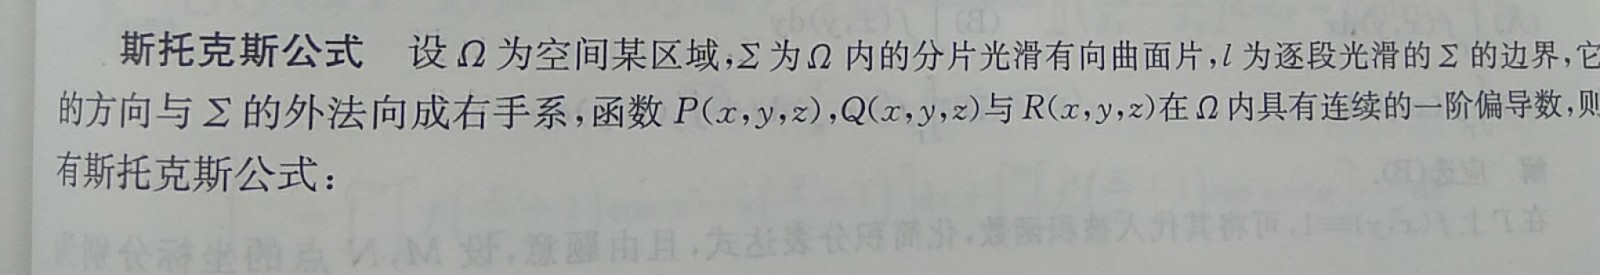
\includegraphics[width=14cm]{9345E7/IMG_20180419_111338.jpg}
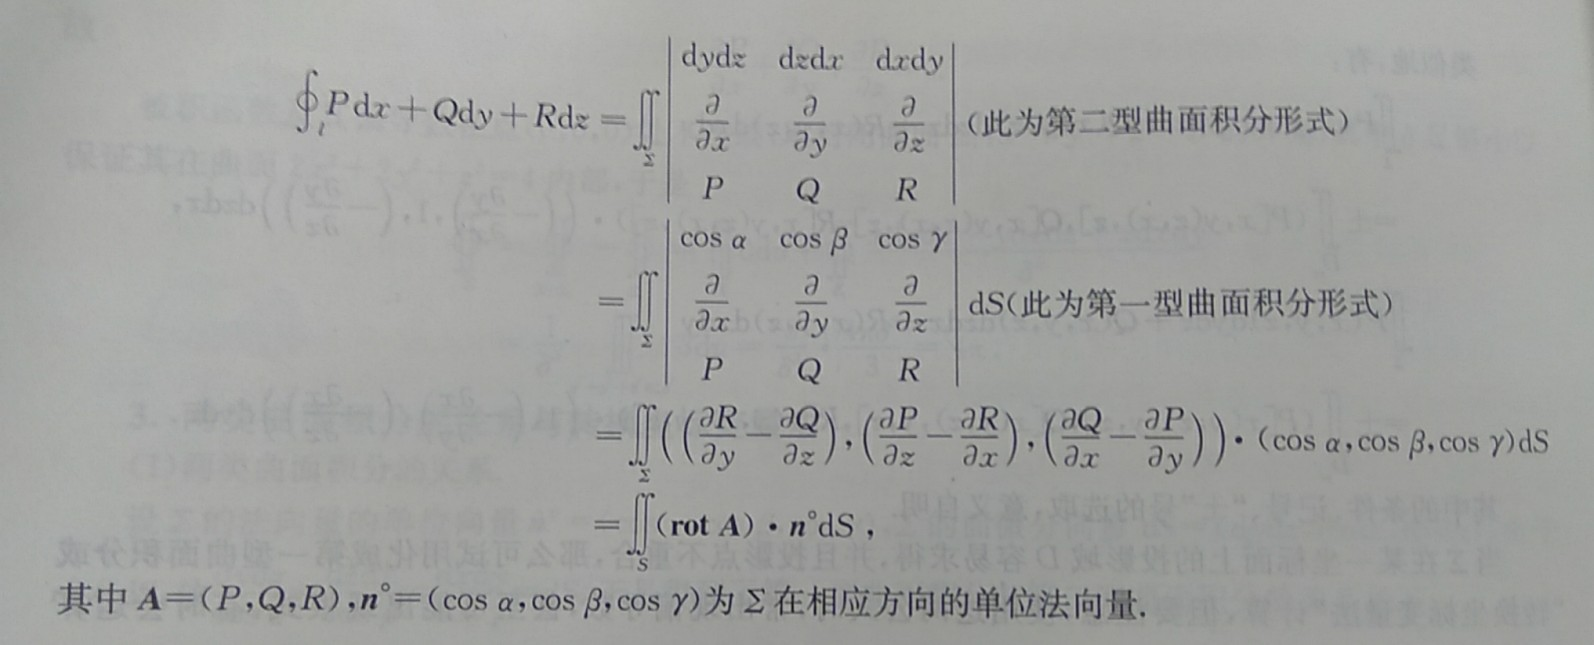
\includegraphics[width=14cm]{9345E7/IMG_20180419_111319.jpg}
\subsection{格林公式}
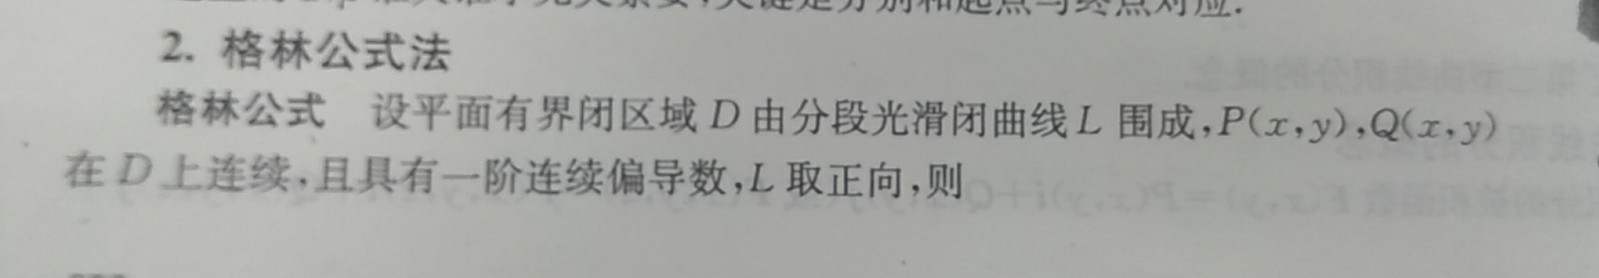
\includegraphics[width=14cm]{9345E7/IMG_20180419_111029.jpg}
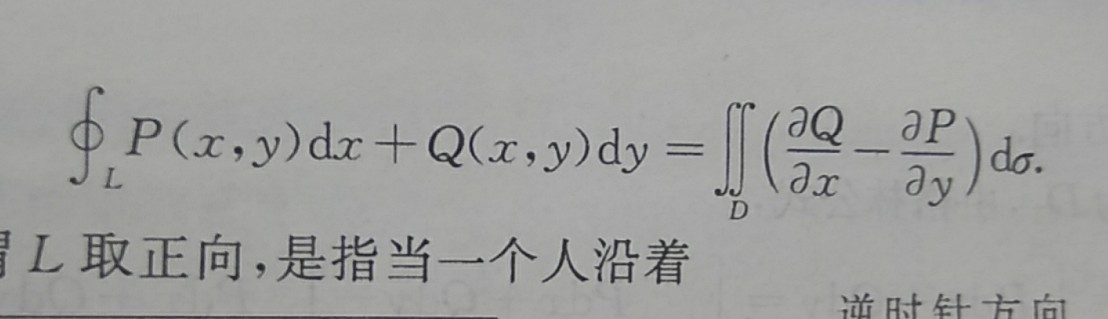
\includegraphics[width=14cm]{9345E7/IMG_20180419_111105.jpg}
\subsection{高斯公式}
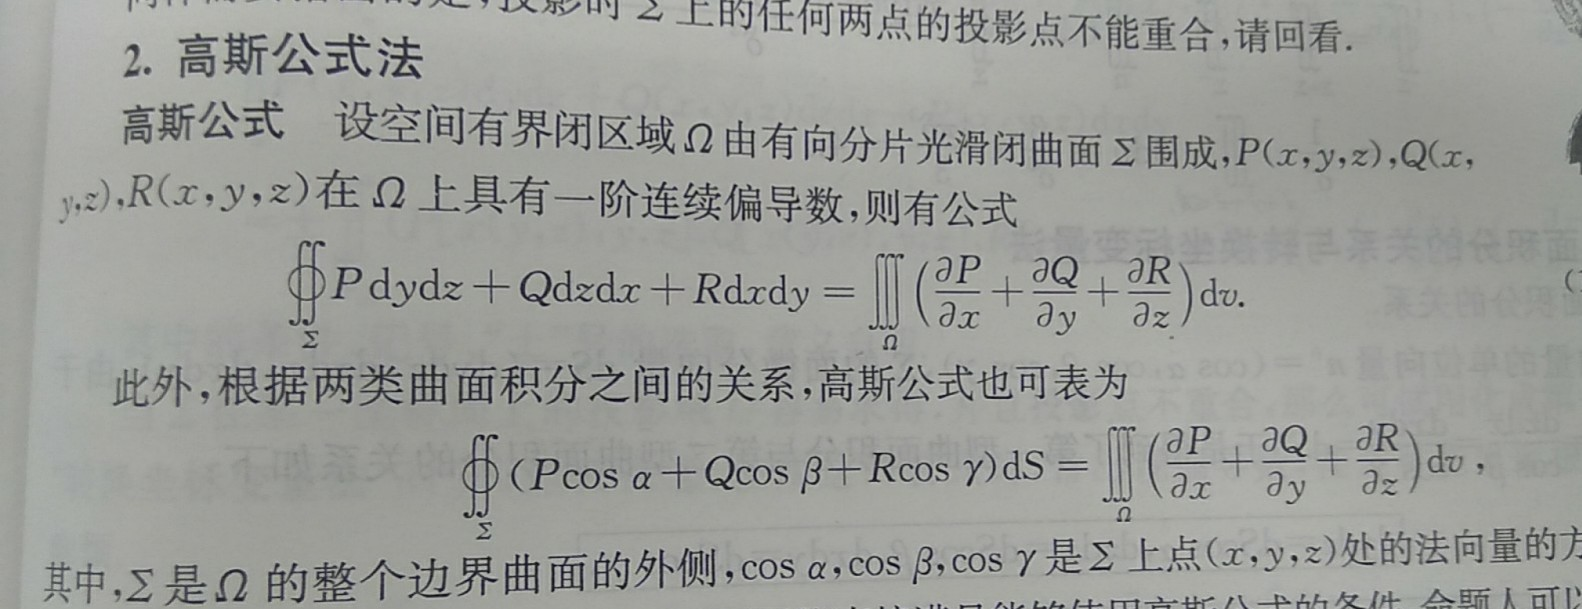
\includegraphics[width=14cm]{9345E7/IMG_20180419_111223.jpg}
\end{document}
